\chapter{Classification}

% ---------- Confusion Matrix ----------
\thispagestyle{classificationstyle}
\section{Confusion Matrix}
\subsection{Confusion Matrix}

% ---------- FPR ----------
\clearpage
\section{FPR}
\subsection{False Positive Rate}
\thispagestyle{classificationstyle}

The False Positive Rate (FPR), also known as the false alarm ratio or fall-out, measures how often negative instances are incorrectly classified as positive in binary classification.

\begin{center}
\tikz{
\node[inner sep=2pt, font=\Large] (a) {
{
$\displaystyle
FPR = \frac{{\color{cyan}FP}}{{\color{cyan}FP} + {{\color{nmlpurple}TN}}}
$
}
};
\draw[-latex,cyan, semithick] ($(a.north)+(1.3,0.05)$) to[bend left=15] node[pos=1, right] {False positives} +(1,.5); 
% \draw[-latex,teal!70!green, semithick] ($(a.south)+(2.1,0.1)$) to[bend right=15] node[pos=1, right] {Mean of targets} +(1,-.5); 
\draw[-latex,nmlpurple, semithick] ($(a.south)+(1.5,-0.05)$) to[bend left=15] node[pos=1, left] {True negatives} +(-1,-.5); 
}
\end{center}

FPR ranges from 0 (no false alarms) to 1 (all predicted positives are incorrect). FPR can also be interpreted as the probability that a negative instance will be incorrectly identified as positive.

\textbf{When to use FPR?}

Use FPR when you need to evaluate how well a classifier avoids false positives, especially when false positives have significant costs, like in medical diagnostics or security systems. It's also useful for understanding the trade-off between true positive rate (sensitivity) and false positive rate.

\coloredboxes{
\item It provides a clear and intuitive measure of a classifier's false positive performance.
\item It helps identify scenarios where the classifier is overly sensitive and prone to false alarms.
}
{
\item FPR does not consider true positive instances.
\item FPR can be sensitive to class imbalance, as it may be easier to achieve a low FPR when the negative class is dominant.
\item FPR doesn't exist in isolation; it's often important to show its relationship with another key metric. (e.g., TPR, Precision, Recall).
}


\clearpage
\thispagestyle{customstyle}


\begin{figure*}[ht!]
    \centering
    \includegraphics[width=0.7\textwidth]{figures/FPR_3d_surface.png}
    % \caption{Caption}
    \label{fig1}
\end{figure*}

\begin{wrapfigure}{r}{0.55\textwidth}
    \centering
    \vspace{-20pt} % Adjust vertical alignment if needed
    \includegraphics[width=0.5\textwidth]{figures/FPR_2d_line_plot.png} % Your figure goes here
\end{wrapfigure}

% Left text with the image on the right
\textbf{Figure 3.1 False Positive Rate.} 
\textbf{Top:}
3D surface illustrating FPR's non-linear relationship with FP and TN. FPR is lowest (blue) when FP is low. It increases (red) as FP increases.
\textbf{Right:}
Shows how FPR decreases hyperbolically as total negative cases increase for fixed FP values. Lower FP maintains better FPR.


\orangebox{%
Did you know that...}
{
In the context of statistical hypothesis testing, the FPR is also known as the "type I error rate" or the probability of rejecting a true null hypothesis.
}

\textbf{FPR alternatives and related metrics}

Other metrics used alongside or instead of FPR include True Positive Rate (TPR), Precision, F1-Score, Receiver Operating Characteristic (ROC AUC), and Specificity.


% ---------- FNR ----------
\clearpage
\section{FNR}
\subsection{False Negative Rate}
\thispagestyle{classificationstyle}

The False Negative Rate (FNR), also known as the miss rate, measures the proportion of actual positive instances incorrectly classified as negative in binary classification.
\begin{center}
\tikz{
\node[inner sep=2pt, font=\Large] (a) {
{
$\displaystyle
FNR = \frac{{\color{cyan}FN}}{{\color{cyan}FN} + {{\color{nmlpurple}TP}}}
$
}
};
\draw[-latex,cyan, semithick] ($(a.north)+(1.3,0.05)$) to[bend left=15] node[pos=1, right] {False negatives} +(1,.5); 
% \draw[-latex,teal!70!green, semithick] ($(a.south)+(2.1,0.1)$) to[bend right=15] node[pos=1, right] {Mean of targets} +(1,-.5); 
\draw[-latex,nmlpurple, semithick] ($(a.south)+(1.5,-0.05)$) to[bend left=15] node[pos=1, left] {True positives} +(-1,-.5); 
}
\end{center}

FNR ranges from 0 (no false negatives) to 1 (all positive instances misclassified). It represents the probability that a positive instance will be incorrectly identified as negative.

\textbf{When to use FNR?}

Use FNR when the cost of missing positive cases is high (e.g., in medical diagnostics or fraud detection) or when you must balance false negatives and false positives.

\coloredboxes{
\item It directly measures the rate of missed positive cases.
\item It is critical in fields where false negatives have severe consequences.
\item Complements True Positive Rate (TPR) in assessing classifier performance.
}
{
\item It doesn't account for true negatives or false positives.
\item It can be misleading in highly imbalanced datasets.
\item It should be considered alongside other metrics for a comprehensive evaluation.
}


\clearpage
\thispagestyle{customstyle}


\begin{figure*}[ht!]
    \centering
    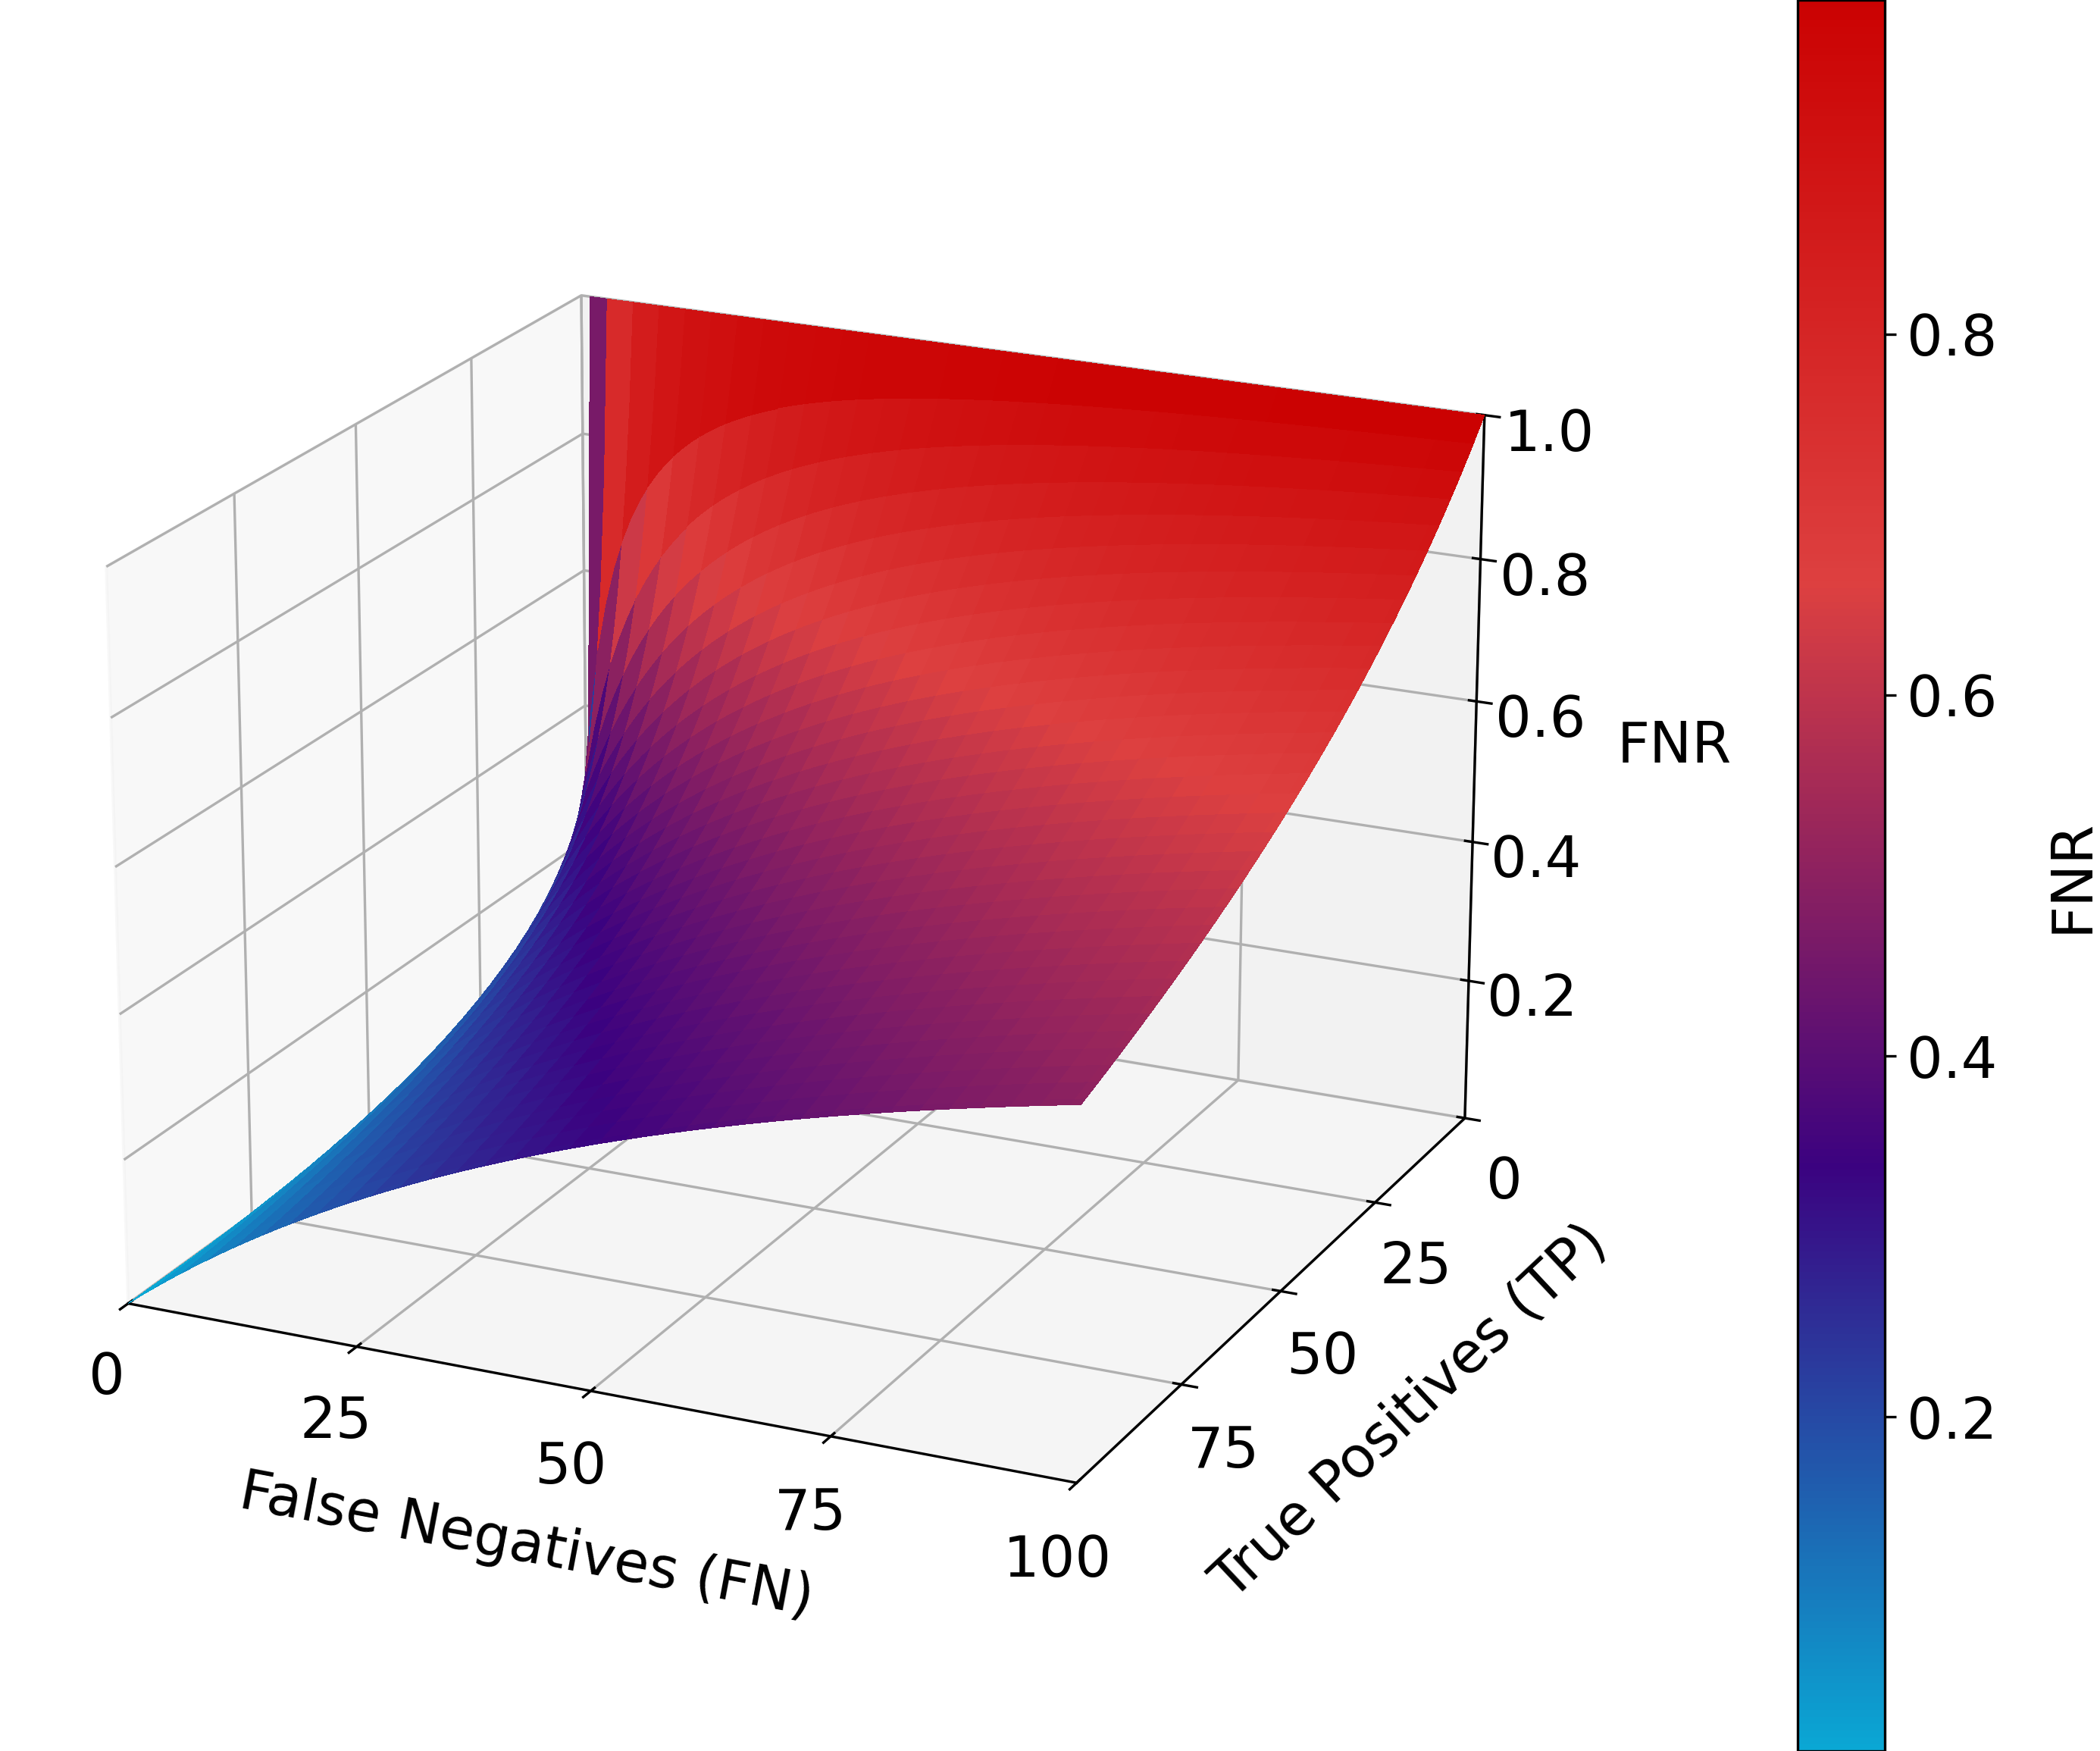
\includegraphics[width=0.7\textwidth]{figures/FNR_3d_surface.png}
    % \caption{Caption}
\end{figure*}

\begin{wrapfigure}{r}{0.55\textwidth}
    \centering
    \vspace{-20pt} % Adjust vertical alignment if needed
    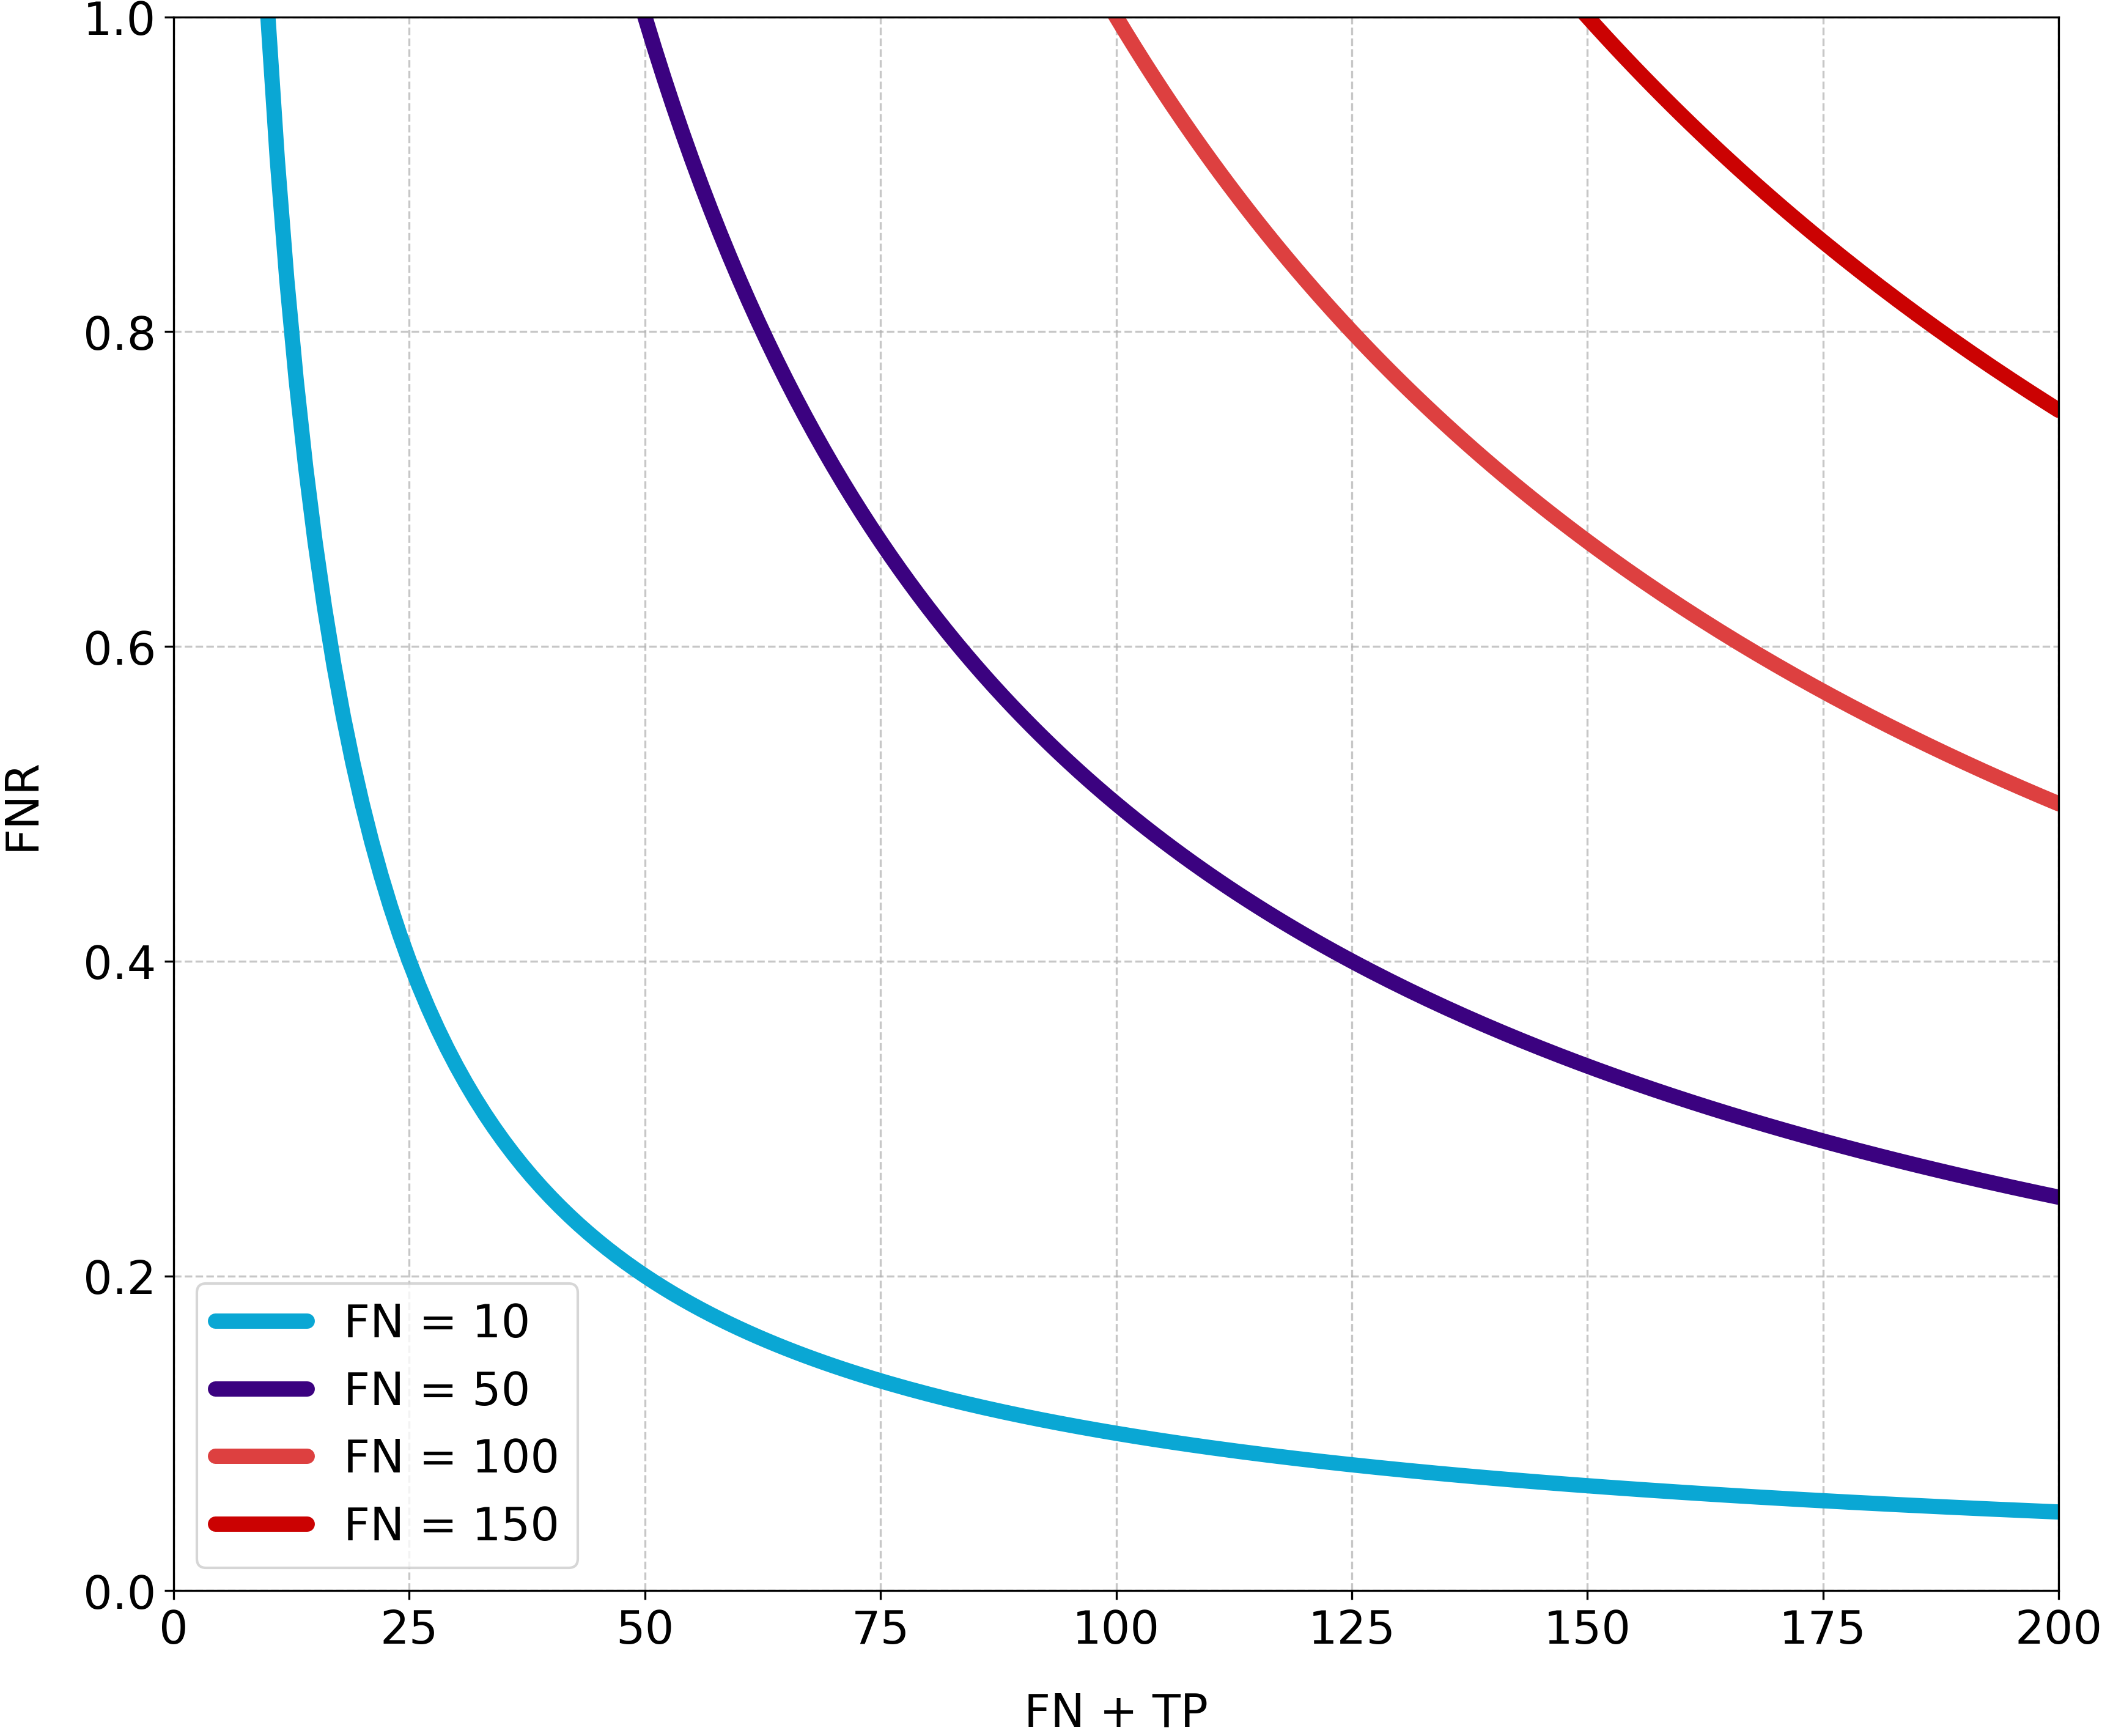
\includegraphics[width=0.5\textwidth]{figures/FNR_2d_line_plot.png} % Your figure goes here
\end{wrapfigure}

% Left text with the image on the right
\textbf{Figure 3.1 False Negative Rate.} 
\textbf{Top:}
3D surface illustrating FNR's non-linear relationship with FN and TP. FNR is lowest (blue) when FN is low. It increases (red) as FN increases.
\textbf{Right:}
Shows how FNR decreases hyperbolically as total positive cases increase for fixed FN values. Lower FN maintains better FNR.


\orangebox{%
Did you know that...}
{
    In hypothesis testing, reducing the False Negative Rate ($\beta$) increases the power of the test ($1 - \beta$), but often at the cost of increasing the False Positive Rate ($\alpha$).
    This demonstrates the inherent trade-off between Type I and Type II errors in statistical testing.
}

\textbf{FNR alternatives and related metrics}

Other metrics used alongside or instead of False Negative Rate (TPR/Recall/Sensitivity), Specificity, Precision, F1-Score, and ROC curve.

% ---------- FNR ----------
\clearpage
\thispagestyle{classificationstyle}
\section{FNR}
\subsection{False Negative Rate}

% ---------- TPR ----------
\clearpage
\thispagestyle{classificationstyle}
\section{TPR}
\subsection{True Positive Rate (Recall/Sensitivity)}

% ---------- TNR ----------
\clearpage
\thispagestyle{classificationstyle}
\section{TNR}
\subsection{True Negative Rate (Specificity)}

% ---------- Accuracy ----------
\clearpage
\thispagestyle{classificationstyle}
\section{Accuracy}
\subsection{Accuracy}

% ---------- Balanced Accuracy ----------
\clearpage
\thispagestyle{classificationstyle}
\section{Balanced Accuracy}
\subsection{Balanced Accuracy}

% ---------- Precision ----------
\clearpage
\thispagestyle{classificationstyle}
\section{Precision}
\subsection{Precision}

% ---------- F1-score ----------
\clearpage
\thispagestyle{classificationstyle}
\section{F1-score}
\subsection{F1-score}

% ---------- F-beta ----------
\clearpage
\thispagestyle{classificationstyle}
\section{F-beta}
\subsection{F-beta}

% ---------- F-beta ----------
\clearpage
\thispagestyle{classificationstyle}
\section{F-beta}
\subsection{F-beta}

% ---------- ROC AUC ----------
\clearpage
\thispagestyle{classificationstyle}
\section{ROC AUC}
\subsection{Area Under the Receiver Operating Characteristic Curve}

% ---------- PR AUC ----------
\clearpage
\thispagestyle{classificationstyle}
\section{PR AUC}
\subsection{Area Under the Precision-Recall Curve}

% ---------- Brier Score Loss ----------
\clearpage
\thispagestyle{classificationstyle}
\section{Brier Score Loss}
\subsection{Brier Score Loss}

% ---------- Log Loss ----------
\clearpage
\thispagestyle{classificationstyle}
\section{Log Loss}
\subsection{Log Loss}

% ---------- Jaccard Score ----------
\clearpage
\thispagestyle{classificationstyle}
\section{Jaccard Score}
\subsection{Jaccard Score}

% ---------- D2 Log Loss Score ----------
\clearpage
\thispagestyle{classificationstyle}
\section{D2 Log Loss Score}
\subsection{D2 Log Loss Score}

% ---------- P4-metric ----------
\clearpage
\thispagestyle{classificationstyle}
\section{P4-metric}
\subsection{P4-metric}

% ---------- Cohen's Kappa ----------
\clearpage
\thispagestyle{classificationstyle}
\section{Cohen's Kappa}
\subsection{Cohen's Kappa}

% ---------- Phi Coefficient ----------
\clearpage
\thispagestyle{classificationstyle}
\section{Phi Coefficient}
\subsection{Phi Coefficient}

% ---------- MCC ----------
\clearpage
\thispagestyle{classificationstyle}
\section{MCC}
\subsection{Matthew's Correlation Coefficient}


% ---------- EC ----------
\clearpage
\thispagestyle{classificationstyle}
\section{EC}
\subsection{Expected Cost}

The Expected Cost (EC) metric is designed to evaluate the performance of decision-making systems. It is the expected value of a cost function that assigns a penalty to each combination of the system's decision and the true class of a sample. 

\begin{center}
\tikz{
\node[inner sep=2pt, font=\Large] (a) {
{
$\displaystyle
EC = \frac{1}{{\color{nmlred}N}} \sum_{t=1}^{N} {\color{nmlpurple}C}({\color{nmlcyan}h_t}, {\color{nmlyellow}d_t})
$
}
};
\draw[-latex,nmlred, semithick] ($(a.south)+(-0.7,0.2)$) to[bend left=30] node[pos=1, left] {number of samples} +(-0.8,-0.5);
\draw[-latex,nmlcyan, semithick] ($(a.north)+(1.3,-0.5)$) to[bend left=30] node[pos=1, right] {true class} +(1.5,0.7);
\draw[-latex,nmlpurple, semithick] ($(a.north)+(0.7,-0.5)$) to[bend right=60] node[pos=1, left] {cost matrix} +(-1.5,0.7);
\draw[-latex,nmlyellow, semithick] ($(a.south)+(2.0,0.5)$) to[bend right=30] node[pos=1, right] {decision} +(1.5,-0.7); 
}
\end{center}

For each possible true class $h$ and decision $d$, a cost $C(h, d)$ is assigned. The expected cost (EC) is then computed by averaging the costs over the test samples. EC does not assume that the set of possible decisions is the set of classes. Instead, the decisions can be the actions that may be taken by the user of the system.


\textbf{When to use EC?}

EC allows assigning specific costs to each combination of true class and predicted decision, making it ideal for applications like finance and healthcare where misclassifications have different consequences. It is highly customizable and effectively handles class imbalance.

\coloredboxes{
\item It can adjust for deployment scenarios by modifying class priors and handling class imbalance.
\item It is flexible and explicitly allows to encode the relative costs of different errors in a transparent manner.
%\item Does not limit the possible decisions to only the class labels.
}
{
\item It's effectiveness depends on well-calibrated model probabilities 
\item Defining an appropriate cost matrix can be challenging and requires knowledge of the application 
%\item EC is less widely adopted, making it harder to compare results with existing benchmarks.
}


\clearpage
\thispagestyle{classificationstyle}

Consider a loan approval scenario with two true classes: $H_1$ (Creditworthy) and $H_2$ (Not Creditworthy), and two decisions: $D_1$ (Approve Loan) and $D_2$ (Reject Loan).

Cost Matrix: Here we have defined a cost matrix C, where we want to heavily penalize approving loans for non-creditworthy customers (false positives).

\begin{center}
\begin{tabular}{|c|c|c|}
\hline
 & $D_1$ (Approve Loan) & $D_2$ (Reject Loan) \\
\hline
$H_1$ (Creditworthy) & $c_{11} =  0$ & $c_{12} = 40$ \\
\hline
$H_2$ (Not Creditworthy) & $c_{21} = 80$ & $c_{22} =  0$ \\
\hline
\end{tabular}
\end{center}

Test Set Example: For each row we calculate the cost $C(h_t, d_t)$ incurred on sample t with true class $h_t$ and system’s decision $d_t$.

\begin{center}
\begin{tabular}{|c|c|c|c|}
\hline
Sample (t)& True Class (h) & Predicted Decision (d) & Cost Incurred \\
\hline
1 & Creditworthy & Approve Loan & $C(h_1, d_1) = 0$ \\
\hline
2 & Not Creditworthy & Approve Loan & $C(h_2, d_2) = 80$ \\
\hline
3 & Creditworthy & Reject Loan & $C(h_3, d_3) = 40$ \\
\hline
\end{tabular}
\end{center}

Taking the mean over these test samples gives us the Expected Cost (EC):
\[
EC = \frac{0 + 80 + 40}{3} = 40
\]

\orangebox{%
Did you know that...}
{
    The EC metric is also known as Expected Prediction Error or Expected Loss. In speech processing, it’s called Detection Cost Function (DCF), used for tasks like speaker verification and evaluations by NIST. It's also equivalent to Negative Expected Utility in decision theory.
}

\textbf{EC alternatives and related metrics}

Metrics like F1-score, AUC, and Precision-Recall are ad hoc, treating all errors equally and lacking control over error trade-offs. However, they excel in interpretation and handling class imbalances. In contrast, Expected Cost (EC) allows explicit control over the cost of different misclassifications.
